\chapter{ARCHITECTURE POUR L'IOT}

\section{Introduction}
  
    \vspace{1em}
   

Les objets se caractérisent 
par 
une capacité
de traitement limitée et par une consommation énergétique réduite pour préserver l’autonomie imposée par une alimentation sur batterie.
Or, les activités les plus consommatrices pour un équipement sont l’émission et la réception de données. 
Pour maximiser l’autonomie des équipements, il faut revoir l’intégralité des protocoles, mais en les calquant sur les architectures existantes pour en assurer la compatibilité. 

La figure~\vref{fig-pile-IoT} reprend un certain nombre d'adaptation protocolaires, à différents niveau du modèle ISO, capable de s'adapter aux caractéristiques des objets contraints. Dans les chapitres suivants nous reviendrons sur ces technologies en partant de la représentation des données pour aller jussqu'aux couches basses.

\begin{figure}[tbp]
\centerline{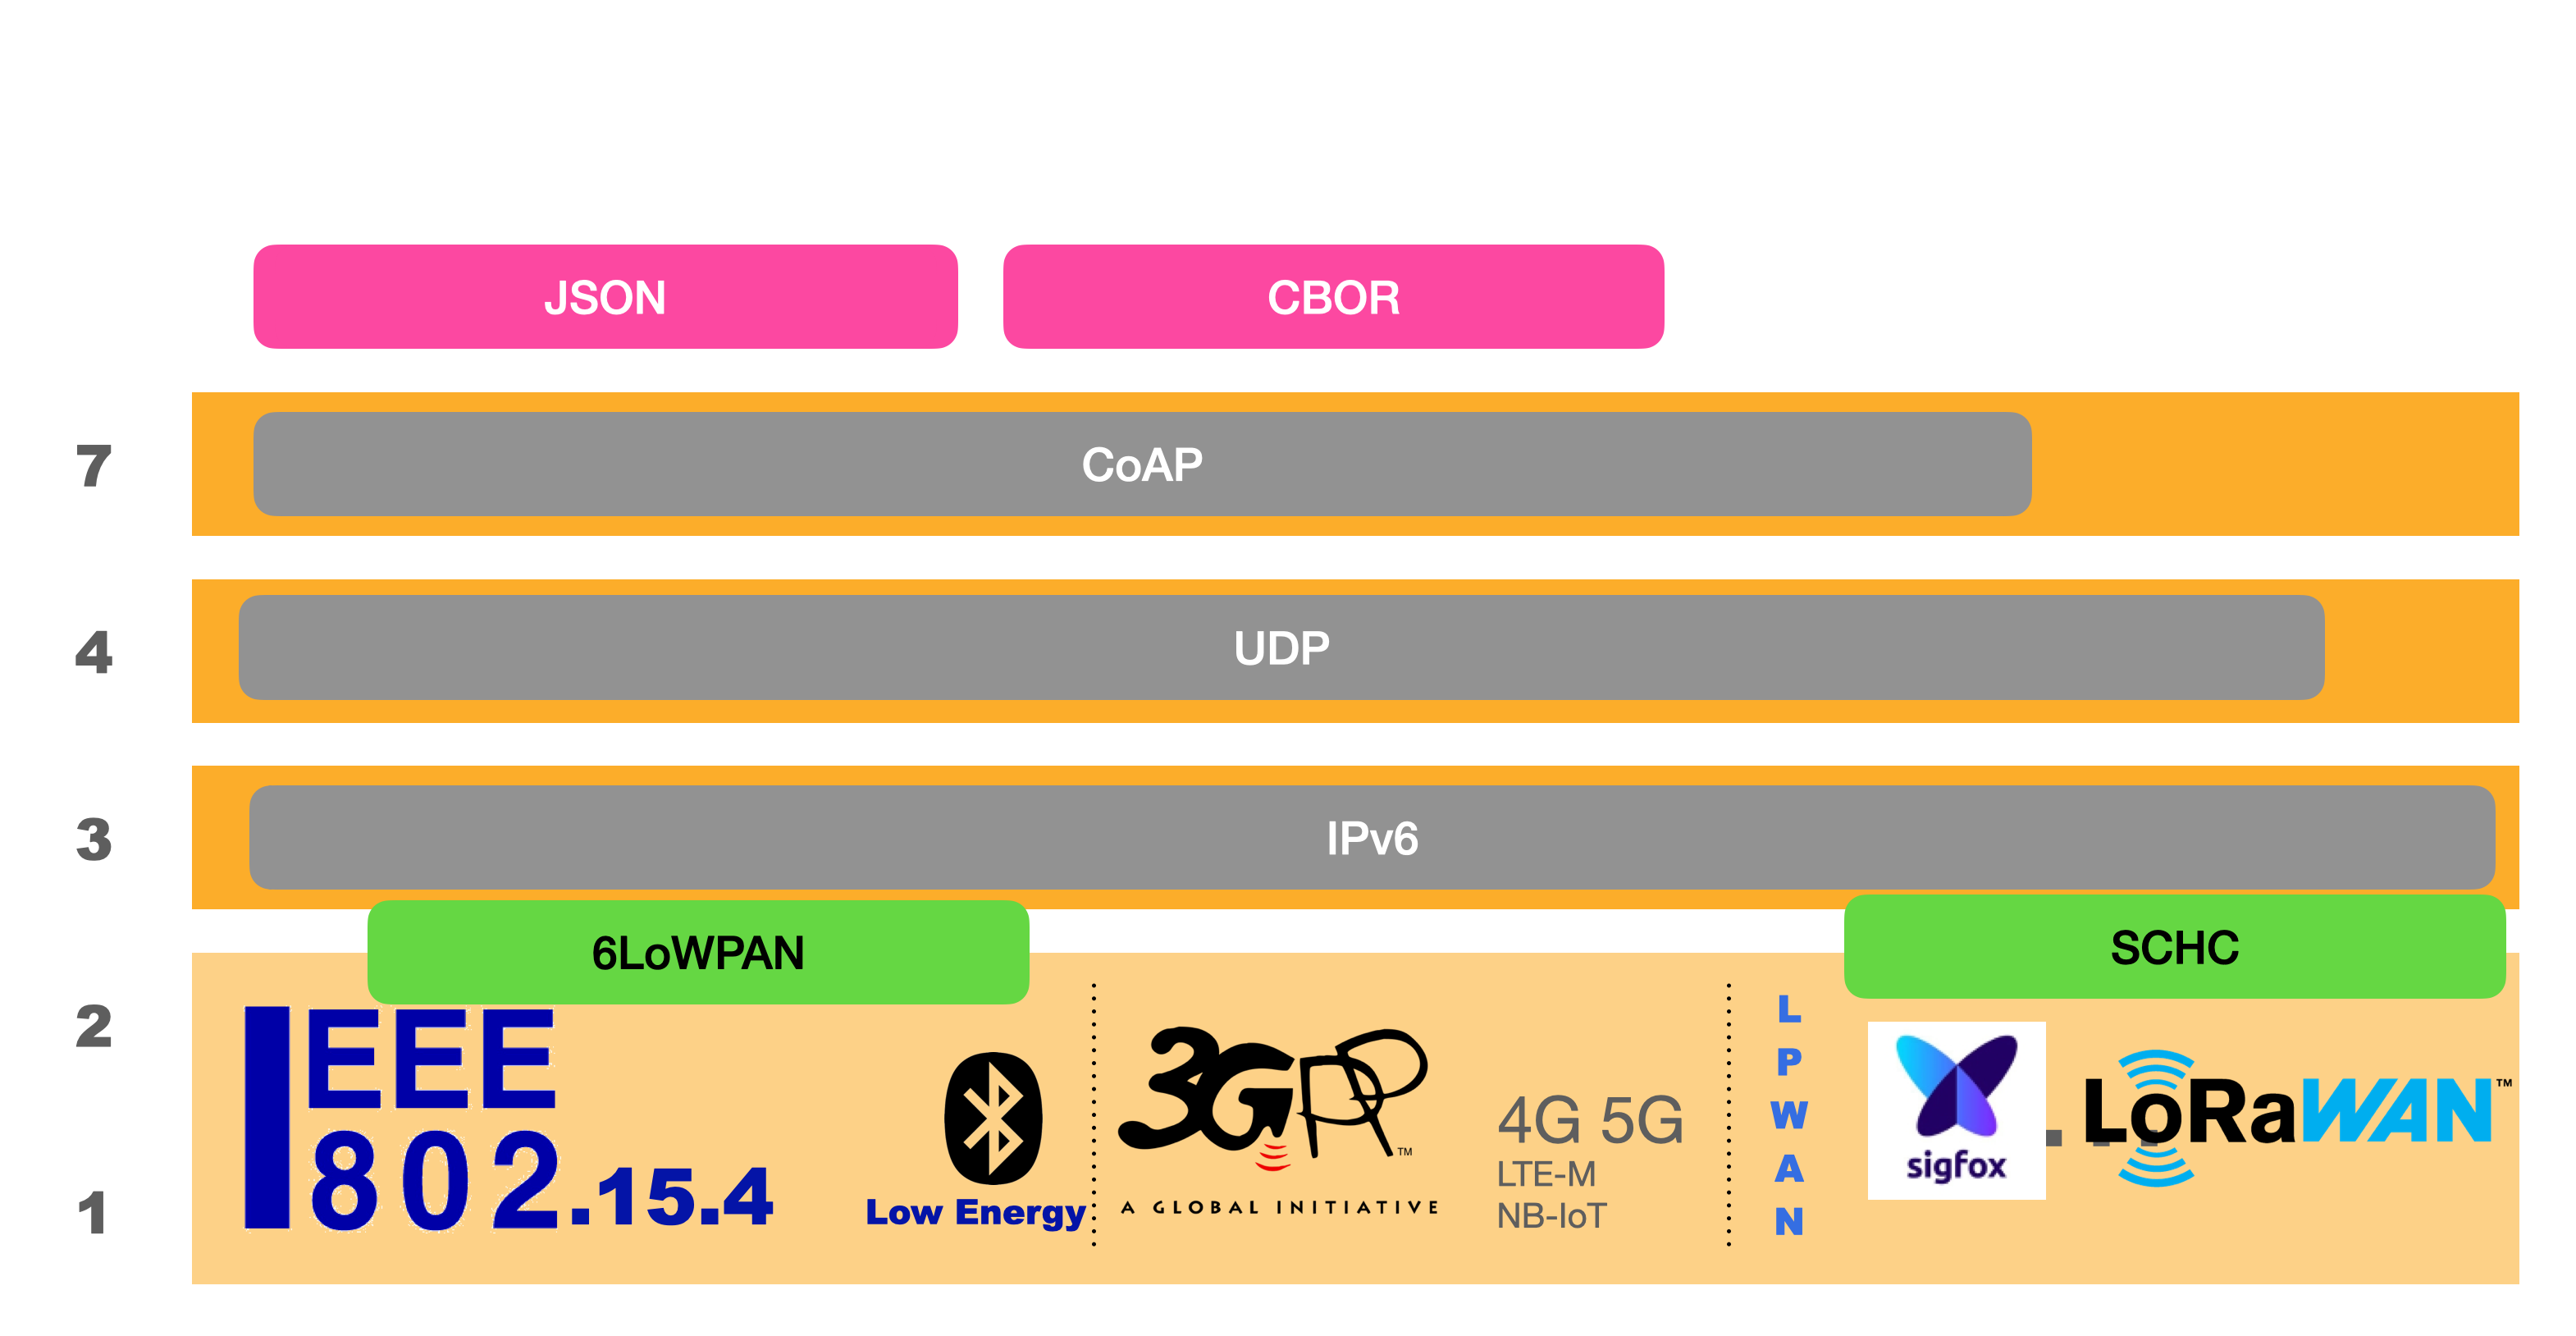
\includegraphics[width=1\columnwidth]{Pictures/Capture17.png}}
\caption{Pile protocolaire de l'IoT}
\label{fig-pile-IoT}
\end{figure}

\section{Topologies}

Les réseaux pour l’internet des objets peuvent être divisés en deux catégories : les topologies maillées (mesh in english) et étoilées (star).


\subsection*{Réseaux Maillés}

Les réseaux maillés, tels que la famille IEEE 802.15.4,  sont une adaptation d’un protocole d’accès Wi-Fi pour préserver l’énergie. La portée de transmission est limitée à 50 mètres pour limiter la consommation d'énergie ; et par conséquent les messages doivent être relayés par d’autres nœuds pour atteindre leur destination.

Le débit est de quelques centaines de kilobits/s et la taille de la trame est de quelques centaines d’octets. 

Ces réseaux sont performants pour transporter des données IoT, mais le protocole de routage, ainsi que le relayage des trames, consomment l’énergie des objets.

\subsection*{Réseaux en Etoile}

Les topologies en étoile ne nécessitent pas de tels mécanismes de routage. Toutes les communications se font avec un point central qui relaie les informations vers la destination.

Les progrès réalisés dans le traitement des signaux permettent d’étendre la portée de transmission à faible puissance. Cette famille de réseaux est appelée réseaux étendus à faible puissance (Low-Power Wide-Area Networks, LPWAN) comme Sigfox, LoRaWAN, ou même du côté de la téléphonie cellulaire avec des évolutions de la norme 4G et une intégration plus complète dans la 5G. Le \rfc{8376} donne, en anglais, un aperçu de ces techniques.


    \vspace{1em}

Avec une puissance de transmission de 25 mW, il est possible de communiquer sur une distance de 3 km en milieu urbain et de 20 km dans un environnement dégagé. Les LPWAN sont compatibles avec les appareils de classe 0 car ils ne nécessitent pas la mise en place d’une pile IP. La figure ci-dessous décrit une architecture typique pour les LPWAN.

\begin{figure}[tbp]
\centerline{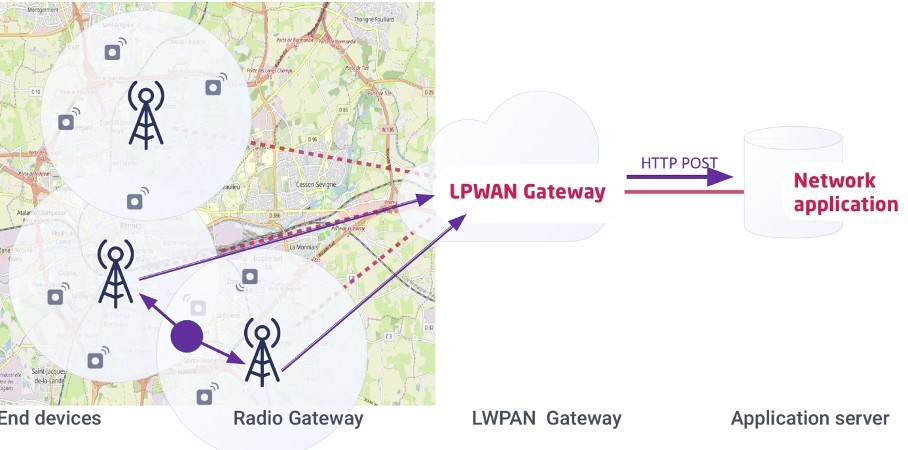
\includegraphics[width=1\columnwidth]{Pictures/TolologieStar.jpg}}
\caption{Architecture simplifiée des réseaux LPWAN}
\label{fig-topo-star}
\end{figure}


L’appareil envoie des données brutes sur le réseau radio. Le signal radio est capté par une ou plusieurs passerelles radio, et la trame est envoyée à une passerelle réseau (LNS - LoRa Network Server- pour les réseaux LoRaWAN, et SCEF - Service Capability Exposure Function Gateway - pour les réseaux 3GPP).

Le propriétaire de l’appareil a associé l’appareil à un connecteur dans le LPWAN Gateway (NGW) qui peut être un URI (Universal Ressource Identifier), une adresse de broker MQTT (Message Queuing Telemetry Transport) ou une Web socket. Lorsque l’appareil envoie des données, il est relié à l’application par ce tunnel.

Certaines technologies telles que LoRaWAN ou Sigfox utilisent des bandes sans licence, imposant un cycle d’utilisation (duty cycle) de 0,1 à 10 \% selon les canaux pour assurer l’équité entre les nœuds, empêchant ainsi qu'un équipement ne monopolise le canal de transmission. Comme cette restriction s’applique également à l’antenne du fournisseur, la communication entre le réseau et l’appareil est considérablement limitée.

L’utilisation principale de ces réseaux LPWAN est la télémétrie où un appareil envoie régulièrement des informations ou une alarme de temps en temps (par exemple des capteurs de température). Le débit et la taille des messages est beaucoup plus réduit que dans le cas de réseaux maillés.

    \vspace{1em}

\section{Niveaux 1 et 2}

 Concernant le niveau 2 , le but est de gagner en énergie lors des transmissions. Déjà on peut dire adieu à Ethernet car cela imposerait d'utiliser l'infrastructure filaire et donc on ne pourrait pas placer les objets où on veut, surtout s'ils se déplacent. Les communications par ondes radio sont privilégiées. 
 
 Pour l'internet des objets, le Wi-Fi est également trop gourmand en énergie. On lui préfère donc une évolution appelée IEEE 802.15.4 qui reprend son principe de fonctionnement mais l'adapte à un faible débit et à des trames de petite taille. En particulier pour économiser l'énergie, la portée est réduite à une dizaine de mètres et il faut généralement utiliser des relais pour atteindre une destination. 
 
 Bluetooth a été adapté pour des objets avec une basse consommation BLE pour bluetooth low energy. 
     \vspace{1em}

 Côté téléphonie cellulaire, les protocoles évoluent pour prendre en compte les objets. La norme 4G a intégrée les communications à plus bas débit. La 5G inclura une classe permettant des communications avec les objets économes en énergie et réduisant les temps de latence. 
 
\section{IP et couches d'adaptation}

  Au niveau 3, on va vers l'utilisation plus massive d'IPv6 puisque la version 4 a son espace d'adressage saturé. la taille de l’adresse est étendue sur 128 bits offrant $2^{96}$ fois plus d’adresses.
  
  \begin{figure}[tbp]
\centerline{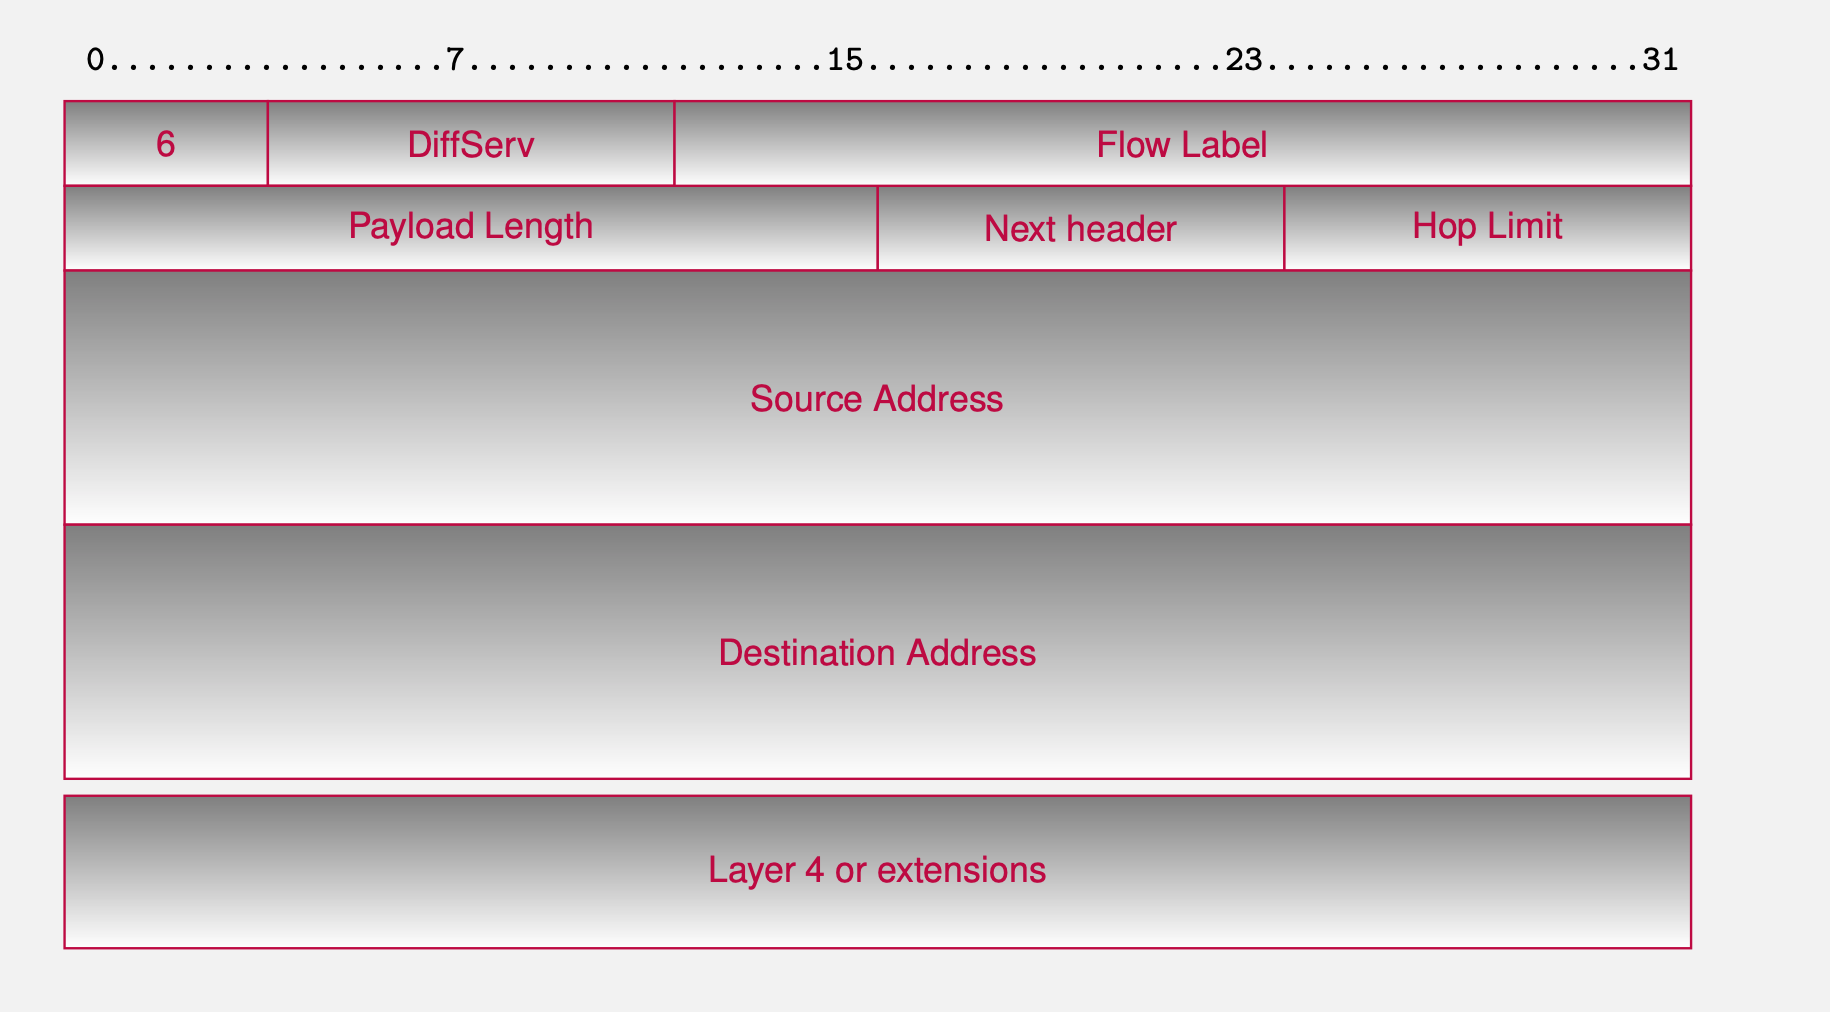
\includegraphics[width=1\columnwidth]{Pictures/Capture18.png}}
\caption{Format d'un en-tête IPv6}
\label{fig-IPv6-header}
\end{figure}

  
  
  
  
  
  Mais, comme on le voir sur la figure~\vref{fig-IPv6-header} IPv6 implique des en-têtes plus grandes, ce qui est gênant car les réseaux de niveau 2 transportent de plus petites trames.
  Une couche d'adaptation entre la couche IP et le niveau 2 est nécessaire puisque les niveaux 2 conçus pour l'internet des objets ne peuvent pas transporter naturellement de grands paquets. Deux actions sont mises en œuvre : compression de la taille des en-têtes pour réduire leur impact, et fragmentation pour découper le paquet en petites trames si la première mesure ne suffit pas. 

Il existe deux grandes familles de couche d'adaptation :

\begin{itemize}
 \item 6LoWPAN \rfc{4944}, \rfc{6282}, qui va intégrer un mécanisme de compression de l'en-tête IPv6 et de fragmentation pour envoyer un gros paquet divisé en petites trames. En effet, dans un réseau maillé, il n'est pas possible de se priver d'informations fournies par la couche IP car les nœuds intermédiaires en ont besoin pour acheminer le message vers le destinataire. 
6LoWPAN est sans état et compresse toutes les en-têtes IPv6 sans configuration. 
\item SCHC (prononcer chic) pour Static Context Header Compression \rfc{8724} va imposer des règles décrivant l'en-tête du message et va envoyer le numéro de la règle en remplacement de l'en-tête. La compression est beaucoup plus importante et peut porter sur plusieurs couches protocolaires. Cependant, pour la mettre en œuvre, il faut avoir une idée des flux qui vont circuler sur le réseau. SCHC est spécifié pour les réseaux en étoile et plus particulièrement les LPWAN.

\end{itemize}

\section{Mise en \oe{}uvre de REST}
  
  Au-dessus on avait vu que comme HTTP était dominant, TCP l'était aussi. Mais pour l'IoT ce n'est pas optimal. En effet TCP/HTTP sont des protocoles complexes qui demandent beaucoup de mémoire. Pour réduire l'impact de la pile protocolaire, l'IETF a défini un nouveau protocole appelé CoAP qui demande que quelques ko pour fonctionner. CoAP repose sur UDP ce qui simplifie encore la mise en oeuvre. 
  
  Pour poursuivre dans l’intégration des objets dans l’internet, le protocole CoAP (Constraint Application Protocol) \rfc{7252} se substitue à HTTP. Il en reprend le mécanisme de nommage, d’utilisation des ressources, et les primitives de manipulation entre un client et un serveur.

La capacité
de traitement
du capteur et son alimentation 
en énergie sont souvent très limitées. 
La grande force de CoAP est d’être :
\begin{itemize}
\item facile à mettre en œuvre. Les mises en œuvre de CoAP nécessitent peu de mémoire ;
\item entièrement compatible avec 
HTTP et il est possible d’aller d’un 
protocole
à l’autre
au travers de 
passerelles
génériques, c’est-à-dire non liées 
à un usage particulier.
\end{itemize}
De ce fait, CoAP va manipuler des ressources, identifiées par des URI. Il est donc possible d'ancrer les données fournies par les objets dans l'écosystème actuel des communications entre ordinateurs, fortement structuré autour des principes REST.

     \vspace{1em}

La sécurité, en particulier 
le chiffrement des données, 
suit aussi les mêmes chemins que l’internet traditionnel. 
Il existe un chiffrement au-dessus d’UDP qui, 
à l’instar
de HTTPS, 
chiffre les échanges.
  
\section{Representation des données}

Pour la structuration des données, XML n'est pas utilisée car il est trop bavard. JSON est beaucoup plus efficace pour transporter des informations structurées. Il existe un équivalent binaire que nous verrons par la suite CBOR qui est beaucoup plus performant, et simple à mettre en oeuvre est compatible avec JSON.

\section {Alternatives à REST}


Il n'est pas obligé de tout mettre en oeuvre tous les protocoles définis par l'IETF. Il est possible également d'y intégrer des protocoles spécifiés pour un métier. 

   \begin{wrapfigure}{r}{7cm}
\centerline{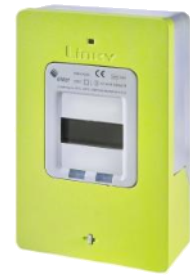
\includegraphics[width=.4\columnwidth]{Pictures/linky.png}}
\end{wrapfigure}

Par exemple, le compteur électrique linky que tous les Français connaissent en implémente qu'une partie. Au lieu d'utiliser CoAP, les électriciens utilisent leurs propres applications suivant la norme DLMS/Cosem. Celle-ci repose sur UDP puis IPv6 et 6LoWPAN et finalement sur une variante de IEEE 802.15.4 adaptée pour transporter l'information sur les câbles électriques.
